\section{Theoretical Basis}

\subsection{Atomar spectra, fine structure and hyperfine structure}

The nucleus of an atom induces an electric field, which binds electrons in orbits around it. Those orbits are quantized according to the boundary conditions the electron's wave function underlies in the Coulomb field. The electron's state is classically described by its principal quantum number $n$ and it's angular momentum $L$. The quantum numbers for all electrons define the atomic spectrum since the absorption and emission of photons depends on the electron's state .

If one considers the intrinsic angular momentum of the electron, the so called spin $S$, one receives a new splitting of the electron states. One can calculate this by adding the spin to the angular momentum of the electron and thus defining a new quantum number, the total angular momentum:

$$ \vec J = \vec L + \vec S $$

The total angular momentum induces a magnetic momentum of the electron, since the electron is a charged particle:

$$\vec \mu_J = \vec \mu_L + \vec \mu_S = - \frac{\mu_B}{\hbar}(g_S\vec S + g_L\vec L) = -\frac{\mu_B}{\hbar}g_J\vec J$$

$\mu_B = \frac{e\hbar}{2m_0} = 9.27\cdot10^{-24}Am^2$ is the Bohr magneton and $g_S \approx 2$, $g_L = 1$ and $g_J$ are the Landé-g-factors. This magnetic momentum then splits up the energy levels of the electrons using the Zeeman-effect. This is called the fine structure of the atom. The energy of a state changes by:

$$ E_{FS} = -\vec\mu_S\cdot\vec B_L $$

If one additionally considers the angular momentum of the nucleus $I$, which results from the nuclear spin of the protons and neutrons, one receives even a new quantum number, the hyperfine total angular momentum:

$$ \vec F = \vec J + \vec I $$

The nuclear spin itself induces a magnetic momentum 

$$\mu_I = \frac{g_I\mu_K}{\hbar}\vec I$$

and a splitting of the energy levels given by:

$$E_{HFS} = -\vec\mu_I\cdot\vec B_J$$

Which leads to the difference between two levels:

$$\Delta E_{HFS} = \frac{1}{2}\underbrace{\frac{g_I\mu_KB_J}{\sqrt{J(J+1)}}}_{=:A}[F(F+1) + J(J+1) + I(I+1)]$$

If the levels are adjacent to each other, this becomes:

\begin{equation} \Delta E_{HFS}(\Delta F = 1) = A\cdot (F+1) \label{A} \end{equation} 


\begin{figure}[H]
\centering 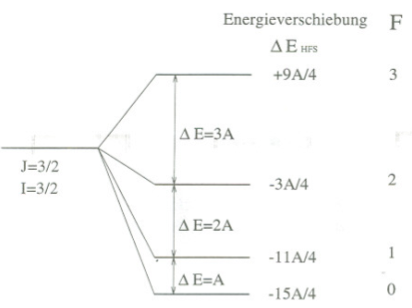
\includegraphics[width=0.75\textwidth]{BilderTheo/HFAufspaltung.png}
\caption{Example of a hyperfine splitting for a J=3/2, I=3/2 state [Ba97]}
\end{figure}


\subsection{Hyperfine structure and Zeeman splitting of Rubidium}

The element used in this experiment is Rubidium. It has two stable isotopes:  $^{85}Rb$ (72.8\%, I = 5/2) and $^{87}Rb$ (27.2\%, I = 3/2). Since it only has one valence electron (the other shells are filled), one can view it as having only one electron. The both states which are relevant for the experiment are $^2S_{1/2}$ and $2P_{1/2}$\footnote{Nomenclature: $^{2S+1}L_J$}. Different states mean different splitting of the energetic levels, which are defined by the hyperfine structure constant A as described in eq. (\ref{A}). Their values are:

\begin{center}
\begin{tabular}[H]{| l | c c |} \hline
A in $\mu$eV & $^{85}Rb$ & $^{87}Rb$ \\ \hline
$^2S_{1/2}$ & 4.185 & 14.13  \\
$^2P_{1/2}$ & 0.499 & 1.692 \\ \hline
\end{tabular}
\end{center}

The hyperfine structure states are still degenerated 2F+1 ($m_F = -F, -F+1, \dots, F$) times and can be splitted by applying an external magnetic field $\vec B$. The energy of the states is then given by:

$$E_B = -\vec\mu_F\vec B \text{\ \ \ \ \ with \ \ \ \ \ } \vec\mu_F = \vec\mu_J + \vec\mu_I$$

Which leads to the difference between two states:

$$\Delta E_B = g_F\mu_BBm_F$$

This is called the Zeeman effect. $g_F$ is the Landé-g-factor of the hyperfine structure. Its value for the Rubidium atom can be taken from the table below. In the case of two neighboring states, both with J = 1/2, one finds:

$$\Delta E _B (\Delta m_F = 1) = \frac{g_J}{2I + 1}\mu_BB$$

Here is a table summarizing all the important quantum numbers and Landé factors of the two relevant Rubidium states:

\begin{center}
\begin{tabular}[H]{| c | c | c c c c c | c c |} \hline
Isotope & I & Term & S & L & J & $g_J$ & F & $g_F$ \\ \hline \hline
 & & & & & & & 2 & -1/3 \\
 & & $^2S_{1/2}$ &1/2 & 0 & 1/2 & 2 &  & \\
 & & & & & & & 3 & 1/3 \\
$^{85}Rb$ & $\frac{5}{2}$ & & & & & & &  \\
 & & & & & & & 2 & -1/3 \\
 & & $^2P_{1/2}$ &1/2 & 1 & 1/2 & 2/3 &  & \\
 & & & & & & & 3 & 1/3 \\ \hline \hline
 
 & & & & & & & 1 & -1/2 \\
 & & $^2S_{1/2}$ &1/2 & 0 & 1/2 & 2 &  & \\
 & & & & & & & 2 & 1/2 \\ 
$^{85}Rb$ & $\frac{3}{2}$ & & & & & & & \\
 & & & & & & & 1 & -1/6 \\
 & & $^2P_{1/2}$ &1/2 & 1 & 1/2 & 2/3 &  & \\
 & & & & & & & 2 & 1/6 \\ \hline
\end{tabular}
\end{center}

\begin{figure}[H]
\centering 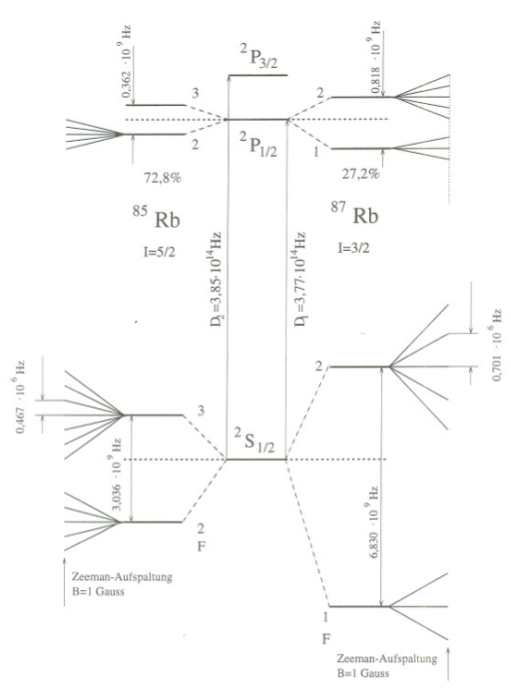
\includegraphics[width = \textwidth]{BilderTheo/RbEnergielevel.png}
\caption{Term diagram of the Rubidium Isotopes (not to scale!) [Ba97]} 
\label{termschema}
\end{figure}

\subsection{Radiative transitions}

As seen in the chapter before, electrons in atoms take discrete energy levels around the nucleus. The transition from one level to another is possible through absorption or emission of electromagnetic radiation (photon), whose energy needs to be the same as the difference in energy between two states. One distinguishes between three different processes:

\begin{itemize}
\item Spontaneous emission
\item Stimulated emission
\item Absorption
\end{itemize}

\begin{figure}[H]
\centering 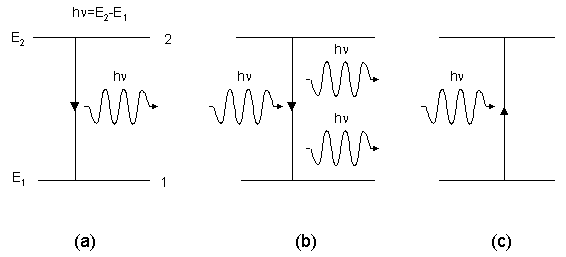
\includegraphics[width = \textwidth]{BilderTheo/absorptionemission.png}
\caption{Spontaneous emission (a), stimulated emission (b) and absorption (c) in a two-level system [asamnet.de]}
\end{figure}

In the following, we will use a two-level system in order to explain the theory clear and simple. Let's say we have one state $\ket{1}$ with energy $E_1$ and one state $\ket{2}$ with energy $E_2$ ($E_1 < E_2$). In this case then, $\ket{1}$ is the ground state and $\ket{2}$ is an excited state. The population of the states is given by the Boltzmann distribution for a certain temperature $T$

$$\frac{N_1}{N_2} = \frac{g_1}{g_2}\exp\left(-\frac{E_2-E_1}{k_BT} \right)$$

where $N_i$ is the population of state $\ket{i}$, $k_B = 1.38\cdot10^{-23} J/K$ the Boltzmann constant and $g_i$ is the degeneracy of level $\ket{i}$, which means how many configurations are possible in a certain state, which for a fine structure level is given by $g_i = 2J +1$, respectively $g_i = 2F+1$ for a hyperfine structure level. The distribution can be changed by absorption or emission by electromagnetic radiation as described above. 

\subsubsection{Selection rules}
\label{sec:selection}

In a system with $\geq 2$ states, not all transitions are possible. They are bound to certain conditions, i.e. one can calculate the transition probability using a transition matrix $|\bra{f}e\vec r\ket{i}|^2$, $\ket{f}$ being the final and $\ket{i}$ the initial state. This element is non-zero for the following transitions in an atom:

\begin{itemize}
\item $\Delta m_J = 0,\pm1$
\item $\Delta J = 0, \pm 1$
\end{itemize}

Also, the following rules apply:

\begin{itemize}
\item transitions $J=0 \to J'=0$ are forbidden
\item $P(\ket{i}) \neq P(\ket{f})$ , P is the Parity of the state
\end{itemize}

This rules for radiative transitions are called selection rules and apply to all electromagnetic dipole transition in an atom or molecule. They are very important for their use in optical pumping, which will be further explained in chapter \ref{sec:1}. 

\subsubsection{Lifetime and line width}

The photon needed for a transition from one level to another actually doesn't need to have the exact frequency corresponding to the energy difference between two states. There are three causes, which broaden the necessary discrete frequency $\nu_0$ to a frequency band $\nu_0 \pm \Delta \nu$.

\begin{enumerate}
\item \textbf{Doppler broadening}

	Because of the velocity the atoms have due to the temperature, the doppler effect leads to a shift of each 	spectral line. If one observes a large number of atoms, the shifts of all the atoms in both directions result in a 	distribution around the original velocity, namely a Maxwell distribution (v being the velocity of an atom in the 	observation direction):
	
	$$ f(v) = \sqrt{\frac{m}{2\pi k_B T}}\exp\left(-\frac{mv^2}{2k_BT}\right) $$
	
	($m$ being the mass of the atoms) which leads to a Gaussian distribution around $\nu_0$ with a FWHM	\footnote{Full width half maximum} of
	
	$$ \Delta \nu_D = \sqrt{\frac{8k_bT\ln2}{mc^2}}\nu_0 $$

	The doppler broadening can be reduced by cooling the atoms.
	
\item \textbf{Pressure broadening}

	Since atoms can scatter each other, their relative phase to the electromagnetic radiation field can suddenly 	change, which also leads to a broadening of the spectral lines. The scattering rate	depends on the 		pressure in the cell, where the atoms are. The FWHM is approximatively given by
	
	$$ \Delta\nu_p = \sqrt{\frac{8}{m\pi k_BT}}pd^2 $$

	$p$ is the pressure in the cell an $d$ is the diameter of an atoms. Obviously, the pressure broadening can 	be reduced by lowering the pressure (but also by augmenting the temperature).
	
\item \textbf{Natural line width}

	Even by strongly decreasing the pressure and the temperature, one finds that the spectral line cannot be 	reduced further at some point. This is called the natural line width, which is a consequence of the finite 		lifetime of a state. Using the uncertainty principle $\Delta E\Delta t \geq \hbar$ one finds that the FWHM of 	the frequency line is limited by
	
	$$ \Delta \nu_0 \geq \frac{1}{2\pi\tau_{sp}} = \frac{e^2}{3\epsilon_0c^3m_e}\nu_0^2 $$
	
	where $\tau_{sp}$ is the lifetime limited by spontaneous emission.

\end{enumerate}

\subsection{Optical pumping}
\label{sec:1}

Optical Pumping roughly means inducing an irregular population distribution in atoms by irradiation of resonant light. This means ''emptying'' occupied states in order to ''fill'' others. \\

As seen in chapter \ref{sec:selection}, the selection rules for electromagnetic dipole transitions include the condition $\Delta m = 0,\pm1$. For the following explanations, it is important to know that $\Delta m$ depends on the polarization of the light relative to the external magnetic field. 

\begin{center}
\begin{tabular}[H]{l c c}
Polarization & Sign & $\Delta m$ \\ \hline
Linear & $\pi$ & 0 \\
Right-Hand Circular & $\sigma^+$ & +1\\
Left-Hand Circular & $\sigma^-$ & -1\\
\end{tabular}
\end{center}

A transition with $\pi$-light is half as probable as one with $\sigma^\pm$-light.

In the picture below, one can see that (naively) $\pi$-light can not induce an irregular distribution, since it is symmetric, but we will later see, that this is also possible. If one uses $\sigma^+$-light, one can pump atoms from the $\ket{S,-1/2}$ to the $\ket{P,+1/2}$ state\footnote{Nomenclature: $\ket{L,m_J}$}. If the atom then finds itself in the latter state, is can spontaneously emit a photon and fall back into either of the two S-states. The probability to fall into the $\ket{S,-1/2}$ state is 66.67\% and 33.33\% to fall into the $\ket{S,+1/2}$ state. The atoms that are in the $\ket{S,-1/2}$ state can then again be pumped by the $\sigma^+$-light until the $\ket{S,-1/2}$ state is empty and all the atoms find themselves (through spontaneous emission) in the $\ket{S,+1/2}$ state. Since transitions from $\ket{S,+1/2}$ to $\ket{S,-1/2}$ are forbidden due to the selection rules, one can imagine the $\ket{S,-1/2}$ state being pumped empty by the $\sigma^+$-light and the $\ket{S,+1/2}$ state being pumped full. This will never happen entirely because of relaxation processes which are described in chapter \ref{sec:relax}.
If an atom is in a $m_J = +1/2$ state, its spin is parallel to an external magnetic field, which means that the atom is being polarized due to optical pumping. 

\begin{figure}[H]
\centering 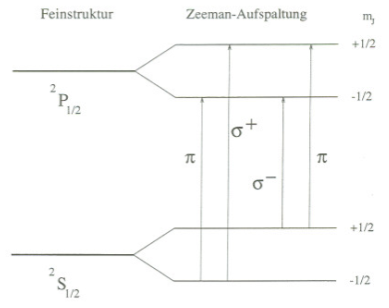
\includegraphics[width = 0.65\textwidth]{BilderTheo/OP-Prinzip.png}
\caption{The transitions depending on the polarization for the both relevant Rb states [Ba97]}
\end{figure}

The polarization is defined by

$$ P =\frac{N_+ - N_-}{N_+ + N_-} =: \frac{n}{N} $$

where $N_\pm$ is the number of atoms in a $m_J = \pm 1/2$ state, $n= N_+ - N_-$ and $N = N_+ + N_-$.\\

The differential equation for the pump process is given by:

$$ \left(\frac{dn}{dt}\right)_{pump} = \frac{N-n}{T_p} $$

where $T_p$ is the pumping time. It is inversely proportional to the pumping light's intensity. The differential equation for relaxation processes is then

$$ \left(\frac{dn}{dt}\right)_{relax} = -\frac{n}{T_R} $$

If one solves those equation, one finally finds that the evolution of the difference in population n in time is

$$ n(t) = n_{max}\left(1-\exp(-t/\tau)\right) $$

with

$$ \frac{1}{\tau} = \frac{1}{T_p} + \frac{1}{T_R} $$

and so the evolution in time of the polarization is

$$P(t) = \frac{n(t)}{N} $$

For Rubidium atoms, we consider the hyperfine structure instead of the fine structure. With a resonant $\sigma^+$-light, one can pump all the atoms into the $\ket{2,2}$\footnote{Nomenclature: $\ket{F,m_F}$} ($^{87}Rb$) or $\ket{3,3}$ state ($^{85}Rb$).\footnote{See picture \ref{termschema} for reference}.

\subsubsection{Relaxation}
\label{sec:relax}

As mentioned above, it is impossible to completely empty one state, since there are relaxation processes which counteract this. Here is a brief description of the most important causes for relaxation in the case of our experiment, i.e. for a spherical cell with a buffer gas (Krypton) which contains the Rubidium. 

\begin{enumerate}
\item \textbf{Diffusion to the cell wall}

	If a polarized Rubidium atom reaches the cell wall, it is exposed to the electromagnetic fields of the ions in 	the wall and its orientation in respect to the external magnetic field is lost, which leads to depolarization.		Depending on the pressure $p$ of the buffer gas, one can see the movement of the atoms as a diffusion. By 	considering this, and the spherical geometry of the cell, one can calculate the relaxation time $T_D$ 		resulting from this process:
	
	$$ \frac{1}{T_D} = \frac{D_0p_0}{p} \left(\frac{2\pi}{d}\right)^2 $$
	
	$D_0 = 0.16 \frac{cm^2}{s}$ is the Diffusion coefficient of Krypton, $p_0$ is the atmospheric pressure and $d	$ is the diameter of the cell.
	
\item \textbf{Buffer gas scattering}

	The buffer gas itself can also scatter the Rubidium atoms and depolarize them. This effect is not very strong, 	since a Rubidium atom has to bounce about $10^9$ times into a Krypton atom in order to lose its 			polarization, but it depends strongly on the pressure inside the cell. The relaxation time which results from 	this scattering is:
	
	$$ \frac{1}{T_R} = N_0\sigma(\braket{v})\braket{v_{rel}}\frac{p}{p_0} $$
	
	Here, $\sigma$ is the depolarization cross section for the averaged velocity of the Rubidium atoms, $v_{rel}$ 	is the relative velocity between the Rubidium and buffer gas atoms and $N_0$ is the density of the buffer 	gas atoms at atmospherical pressure.

\item \textbf{Spin exchange}

	Naturally, Rubidium atoms can also collide with each other. In this case, the valence electrons of the 		Rubidium atoms can exchange spins. Even though this doesn't change the total polarization of all atoms, it 	decouples the nuclear and electron spin, which leads to a faster rebalancing between the two hyperfine 	states $F = I \pm \frac{1}{2}$.

\end{enumerate}

\clearpage






















